\documentclass[table, usenames, svgnames, dvipsnames]{beamer}
\usepackage{listings}
\usepackage{beamerthemeshadow}
\usepackage[latin1]{inputenc}
\usepackage[absolute,overlay]{textpos}
\usepackage{array}

% Coisas adicionadas pelo Alberto.
\usepackage{proof}
\usepackage{easylist}
% \usepackage[portuguese]{babel}
\usepackage{amsmath}
\usepackage[round]{natbib}

\usetheme{Rochester}
%\usetheme{Luebeck}
\usecolortheme{rose}

\setbeamerfont{frametitle}{size=\normalsize}
\setbeamerfont{title}{size=\normalsize}
\beamertemplatenavigationsymbolsempty

\setbeamertemplate{navigation symbols}{}
\setbeamertemplate{footline}{}

\DeclareGraphicsExtensions{.pdf,.jpg,.png} % compilamos apenas com pdflatex
\graphicspath{{.}{./figuras/}} % caminho onde as figuras estarao disponiveis

\setlength{\TPHorizModule}{1mm}

\setlength{\TPVertModule}{1mm}
\newcommand{\MyLogo}{%
\begin{textblock}{}(118.5, 2.5)
   
\includegraphics[width=0.7cm]{figuras/ime-mod2.png}
\end{textblock}
}

\title{\footnotesize Express�es Aritm�ticas Tipadas e C�lculo Lambda Simplesmente Tipado}

% \usepackage{framed} % utilizado para codigo fonte
\definecolor{shadecolor}{named}{LightGray}

\usepackage[portuguese]{babel}

% ---------------------------------------------------------------------------- %
% T�tulo
% ---------------------------------------------------------------------------- %

\subtitle{}
\date{}

% ---------------------------------------------------------------------------- %
\begin{document}
% ---------------------------------------------------------------------------- %

% ---------------------------------------------------------------------------- %
% Primeira p�gina: slide 0
% --------------------------------------------------------------------------- - %
\begin{frame}
   \centering
   \textsc{Universidade Federal de Santa Maria}\\
   \textsc{Programa de P�s-Gradua��o em Inform�tica - PPGI}\\
   \vspace{15pt}
   \titlepage
   \vspace{-60pt}
   \begin{center}
      \textsc{Linguagens de Programa��o -- ELC921}\\
      \textsc{Prof� Dr� Juliana Kaiser Vizzotto}\\
      \hfill\\
      \textsc{Alunos:} Alberto Kummer, Camila Nogueira, Daniel di Domenico, Fernando Campagnolo, Jos� Puiati
   \end{center}
\end{frame}

\begin{frame}
   \frametitle{8.1 Tipos (Express�es Aritm�ticas Tipadas)}
   \begin{itemize}
      \item Avalia��o de termos sem tipos:
         \begin{itemize}
            \item [$\checkmark$] Resulta em um valor (\texttt{true}, \texttt{false} ou \texttt{nv} [\texttt{0} ou \texttt{succ nv}]).
            \item [$\checkmark$] Ou trava em algum est�gio da avalia��o no qual nenhuma regra de avalia��o se aplica (\texttt{pred false}).
         \end{itemize}
   \end{itemize}
\end{frame}

\begin{frame}
   \frametitle{8.1 Tipos (Express�es Aritm�ticas Tipadas)}
   \begin{itemize}
      \item Objetivo dos tipos:
         \begin{itemize}
            \item [$\checkmark$] Identificar termos com erros que ir�o ocasionar um travamento antes de avali�-los.
            \item [$\checkmark$] Tipos criados: \texttt{Bool} (\textit{booleans}) e \texttt{Nat} (naturais).
            \item [$\checkmark$] De forma est�tica: \texttt{t : T} (\texttt{t} possui tipo \texttt{T}) indica que \texttt{t} ir� avaliar para um valor de forma correta (sem travamento) dispensando a necessidade de avali�-lo.
            \item [$\checkmark$] An�lise conservadora: usa apenas a informa��o est�tica, n�o permitindo express�es como \texttt{if true then 0 else false}, mesmo que elas n�o ocasionem um travamento.
         \end{itemize}
   \end{itemize}
\end{frame}

\begin{frame}
   \frametitle{8.2 Rela��o dos tipos}
   \begin{itemize}
      \item Conjunto de regras de infer�ncia que atribuem tipos ao termos, onde \texttt{t : T} (o termo \texttt{t} tem tipo \texttt{T}):
   \end{itemize}
   \begin{block}{Regras de tipos para booleans}
      \begin{align*}
         & \texttt{true : Bool} & & (\textsc{T-True})\\
         & \\
         & \texttt{false : Bool} & & (\textsc{T-False})\\
         & \\
         & \mbox{\infer{\texttt{if t$_1$ then t$_2$ else t$_3$ : T}}{\texttt{t$_1$ : Bool} & &  \texttt{t$_2$ : T} &  & \texttt{t$_3$ : T}}} & & \textsc{(T-If)}
      \end{align*}
   \end{block}
   Adaptado de \citep{pierce}.
\end{frame}

\begin{frame}
   \frametitle{8.2 Rela��o dos tipos}
   \begin{block}{Regras de tipos para n�meros}
      \footnotesize
      \begin{align*}
         & \texttt{0 : Nat} & & \textsc{(T-Zero)}\\
         & \\
         & \mbox{\infer{\texttt{succ t$_1$ : Nat}}{\texttt{t$_1$ : Nat}}  } & & \textsc{(T-Succ)}\\
         & \\
         & \mbox{\infer{\texttt{pred t$_1$ : Nat}}{\texttt{t$_1$ : Nat}}  } & & \textsc{(T-Pred)}\\
         & \\
         & \mbox{\infer{\texttt{iszero t$_1$ : Bool}}{\texttt{t$_1$ : Nat}}  } & & \textsc{(T-IsZero)}\\
      \end{align*}
   \end{block}
   \normalsize
   Adaptado de \citep{pierce}.
\end{frame}

\begin{frame}
   \frametitle{8.2 Rela��o dos tipos}
   \begin{itemize}
      \item Deriva��o de tipos:
      \begin{itemize}
         \item [$\checkmark$] �rvores de inst�ncias de tipos.
         \item [$\checkmark$] Exemplo: \texttt{if iszero 0 then 0 else pred 0}.
      \end{itemize}
   \end{itemize}
\end{frame}

\begin{frame}
   \frametitle{8.2 Rela��o dos tipos}
   \begin{theorem}[\textsc{Teorema da unicidade dos tipos}]
      Indica que, se um termo possui um tipo, esse tipo � �nico e existe apenas uma
      regra de infer�ncia que deriva a sua constru��o.
   \end{theorem}
\end{frame}


\begin{frame}
   \frametitle{8.3 Seguran�a = Progresso + Preserva��o}
   \begin{itemize}
      \item Garantias que a avalia��o de um programa bem tipado n�o travar�.
      \item Dois pilares da seguran�a:
      \begin{itemize}
         \item [$\checkmark$] \textbf{Progresso:} termos bem tipados s�o avaliados completamente (at� sua forma normal).
         \item [$\checkmark$] \textbf{Preserva��o:} um passo de avalia��o de um termo bem tipado resulta noutro termo igualmente bem tipado.
      \end{itemize}
      \item No decorrer do Cap�tulo 8.3, \cite{pierce} mostra exemplos de Progresso e Conserva��o, onde os termos s�o classificados em alguma regra de infer�ncia (como \textsc{T-True, T-If} e \textsc{T-Succ}) e � aplicada alguma regra de avalia��o a ele (\textsc{E-IfTrue, E-If, E-Succ, }\ldots).
   \end{itemize}
\end{frame}

\begin{frame}
   \frametitle{8.3.1 Formas Can�nicas}
   \footnotesize
   \begin{lemma}[\textsc{Formas Can�nicas} \texttt{I}]
      Se \texttt{v} � um valor do tipo \texttt{Bool} ent�o v � \texttt{true} ou
      \texttt{false}.
      \begin{align*}
         \text{t} \qquad & ::= & &\\
         & \text{\texttt{true}} & \text{valor ``verdadeiro''}\\
         & \text{\texttt{false}} & \text{valor ``falso''}\\
      \end{align*}
   \end{lemma}
   \begin{lemma}[\textsc{Formas Can�nicas} \texttt{II}]
      Se \texttt{v} � um valor do tipo \texttt{Nat} ent�o v � um valor num�rico
      conforme a gram�tica:
      \begin{align*}
         \text{v} \qquad & ::= \ldots & \\
         & \text{nv} & \text{valor num�rico}\\
         \text{nv} \qquad & ::= & \\
         & \text{\texttt{0}} & \text{valor ``zero''}\\
         & \text{\texttt{succ nv}} & \text{sucessor}
      \end{align*}
   \end{lemma}
\end{frame}

\begin{frame}
   \frametitle{8.2.1 Invers�o da Rela��o de Tipos}
   \begin{lemma}[Invers�o da Rela��o de Tipos]
      \begin{enumerate}
         \item Se \texttt{true : R} ent�o \texttt{R = Bool}. \label{invtipos:true}
         \item Se \texttt{false : R} ent�o \texttt{R = Bool}. \label{invtipos:false}
         \item Se \texttt{if t1 then t2 else t3 : R}, ent�o \texttt{t1 : Bool},
            \texttt{t2 : R}, e \texttt{t3 : R}.
         \item Se \texttt{0 : R}, ent�o \texttt{R = Nat}. \label{invtipos:zero}
         \item Se \texttt{succ t1 : R}, ent�o \texttt{R = Nat} e \texttt{t1 : Nat}.
         \item Se \texttt{pred t1 : R}, ent�o \texttt{R = Nat} e \texttt{t1 : Nat}.
         \item Se \texttt{iszero t1 : R}, ent�o \texttt{R = Bool} e \texttt{t1 : Nat}.
      \end{enumerate}
   \end{lemma}
   \textbf{Prova: } Imediato a partir das Formas Can�nicas.
\end{frame}

\begin{frame}
   \frametitle{8.3.2 Teorema: Progresso}
   \begin{block}{}
      Suponha \texttt{t} um termo bem tipado. Ent�o ou \texttt{t} � um valor ou ele ser� avaliado (\texttt{t} $\rightarrow$ \texttt{t'}).
   \end{block}
   \begin{itemize}
      \item Por indu��o, \textsc{T-True}, \textsc{T-Zero} e \textsc{T-False} s�o
         casos diretos: itens \ref{invtipos:true}, \ref{invtipos:zero} e
         \ref{invtipos:false} do Lema de Rela��o de Tipos, respectivamente.
      \item \texttt{T-If}:
      \begin{itemize}
         \item [$\checkmark$] se a guarda do \texttt{if} � um valor ent�o ele ser�
         \texttt{true} ou \texttt{false} conforme as Formas Can�nicas e uma das seguintes regras ser�o aplicadas: \texttt{E-IfTrue} ou \texttt{E-IfFalse}.
         \item [$\checkmark$] sen�o \texttt{t} $\rightarrow$ \texttt{t'} e aplica-se \texttt{T-If} sob a guarda avaliada \texttt{t'}.
      \end{itemize}
      \item \texttt{T-Succ}:
         \begin{itemize}
            \item se \texttt{t} for um valor ent�o ele � do tipo num�rico (\texttt{Nat}) e, segundo as Formas Can�nicas, avalia para \texttt{0} ou \texttt{succ nv}
            \item sen�o \texttt{t} $\rightarrow$ \texttt{t'} via \textsc{E-Succ}.
         \end{itemize}
   \end{itemize}
\end{frame}

\begin{frame}
   \frametitle{8.3.2 Teorema: Progresso}
   \begin{block}{}
      Suponha \texttt{t} um termo bem tipado. Ent�o ou \texttt{t} � um valor ou ele ser� avaliado (\texttt{t} $\rightarrow$ \texttt{t'}).
   \end{block}
   \begin{itemize}
      \item \texttt{T-Pred}:
         \begin{itemize}
            \item [$\checkmark$] se \texttt{t} for um valor ent�o ele � do tipo num�rico (\texttt{Nat}) e pode ser avaliado por uma das seguintes regras:
            \textsc{E-PredZero} ou \textsc{E-PredSucc} e
            \begin{itemize}
               \item [] \texttt{pred t : R} ent�o \texttt{R = Nat} e \texttt{T = Nat}
            \end{itemize}
            \item [$\checkmark$] sen�o \texttt{t} $\rightarrow$ \texttt{t'} e \texttt{pred t} $\rightarrow$ \texttt{pred t'}.
         \end{itemize}
      \item \texttt{T-IsZero}
      \begin{itemize}
         \item [$\checkmark$] Mesmas condi��es de \textsc{T-Pred} com a ressalva
         de que as regras aplic�veis a \texttt{t} s�o \textsc{E-IszeroZero}, \textsc{E-IszeroSucc} e \textsc{E-IsZero}
      \end{itemize}
   \end{itemize}
\end{frame}

\begin{frame}
   \frametitle{8.3.3 Teorema: Preserva��o}
   \begin{block}{}
      Suponha \texttt{t : T} e \texttt{t} $\rightarrow$ \texttt{t'}. Ent�o
      \texttt{t' : T}.
   \end{block}
   \begin{itemize}
      \item \textsc{T-True, T-False} e \textsc{T-Zero}:
         \begin{itemize}
            \item [$\checkmark$] t � um valor e o teorema n�o se aplica.
         \end{itemize}
      \item \textsc{T-If}
      \begin{itemize}
         \item [$\checkmark$] {\footnotesize \texttt{t = if t1 then t2 else t3  t1 : Bool t2 : T   t3: T}}
	 \item [$\checkmark$] De acordo com as regras de deriva��o, \textsc{T-If} pode ser avaliado por \textsc{E-IfTrue}, \textsc{E-IfFalse}
	          ou \textsc{E-If}: 
	 \begin{itemize}
	    \item [$\phi$] Subcaso \textsc{E-IfTrue}: \texttt{t$_1$ = true}, \texttt{t' = t$_2$}: de acordo com a regra \texttt{t' = t$_2$},
	                   ent�o \texttt{t'} � do mesmo tipo que \texttt{t$_2$}. (\textsc{E-IfFalse}, de maneira semelhante) 
	    \item [$\phi$] Subcaso \textsc{E-If}: \texttt{t$_1$ $\rightarrow$ t$_1$'} \texttt{t' = if t$_1$' then t$_2$ else t$_3$}
% 	    \begin{itemize}
	      \item [$\phi$] Por deriva��o: \texttt{t$_1$ : Bool}
	      \item [$\phi$] Por indu��o: \texttt{t$_1$' : Bool}
	      \item [$\phi$] \texttt{if t$_1$' then $t_2$ else $t_3$: T; t' : T} \textsc{(T-If)}.
% 	    \end{itemize}  
	 \end{itemize}
      \end{itemize} 
   \end{itemize}
\end{frame}

\begin{frame}
   \frametitle{8.3.3 Teorema: Preserva��o}
   \begin{itemize}
      \item Caso \textsc{T-Succ}: \texttt{t = succ t$_1$ T = Nat t$_1$: Nat}
         \begin{itemize}
            \item [$\checkmark$] Observando as Formas Can�nicas, podemos aplicar a regra \textsc{E-Succ} que deriva \texttt{t} 
            $\rightarrow$ \texttt{t'}. Ent�o \texttt{t}$_1 \rightarrow$ \texttt{t$_1$'}. Sabendo que \texttt{t$_1$ : Nat}, ent�o 
            \texttt{t$_1$' : Nat}, obtendo \texttt{succ t$_1$': Nat}, isto �, \texttt{t' : T} \textsc{(T-Succ)}
         \end{itemize}
    \end{itemize}  
\end{frame}



%inicio jessica
\begin{frame}
\frametitle{Tipos de Fun��es}
\begin{itemize}
\item Para construir um tipo que combine booleanos com primitivas do c�lculo lambda � preciso
adicionar uma classifica��o para os termos cuja avalia��o resulta em uma fun��o;
\item A fim de ter certeza de que a fun��o ir� se comportar corretamente quando for chamada, precisamos manter o controle de qual o tipo de argumento que ela espera.
\end{itemize}
\end{frame}

\begin{frame}
\frametitle{Tipos de Funcoes}
\begin{itemize}
\item Para manter esta informa��o, podemos utilizar um novo tipo:
\end{itemize}
\begin{eqnarray*}
    & T ::= \\
    && Bool \\
    && T \to T\\
\end{eqnarray*}
\end{frame}

\begin{frame}
\frametitle{Tipos de Fun��es}
\begin{itemize}
\item Exemplo:
\end{itemize}
\begin{eqnarray*}
    & Bool \to Bool \\
    & (Bool \to Bool) \to (Bool \to Bool) \\
\end{eqnarray*}
\end{frame}

\begin{frame}
\frametitle{Rela��o  de Tipos}
\begin{itemize}
\item Para saber o tipo de uma abstra��o como \textcolor{red}{$"\lambda x.t"$}, precisamos calcular o que acontece quando essa abstra��o � aplicada a algum argumento;
\item Abordagem utilizada agora: anotar a abstra��o com o tipo esperado para seus argumentos.
\item Exemplo: \textcolor{red}{$"\lambda x.t"$} ser� \textcolor{red}{$"\lambda x:T1 .t2"$}
\end{itemize}
\end{frame}

\begin{frame}
\frametitle{Rela��o  de Tipos}
\begin{itemize}
\item Termos podem conter abstra��es aninhadas. Com isso em mente, utilizaremos $\Gamma \vdash t : T$ onde $\Gamma$ � um conjunto com as vari�veis livres de t e seus respectivos tipos. Sendo assim, a regra de tipo para abstra��es ser�:
\end{itemize}
 \begin{center}
{\huge $\frac{\Gamma ,x\ :\ T_1 \vdash t_2\  :\  T_2}{\Gamma\  \vdash\  \lambda x\  :\ T_1 .t_2\  :\  T_1 \to T_2}$}  $\qquad (T-Abs)$
 \end{center}
\end{frame}

\begin{frame}
\frametitle{Rela��o  de Tipos}
\begin{itemize}
\item A regra para vari�vel �:
\end{itemize}
 \begin{center}
{\huge $\frac{x:T\ \in\ \Gamma}{\Gamma\ \vdash\ x\ :\ T}$}  $\qquad (T-Var)$
 \end{center}
 \begin{itemize}
\item A regra para aplica��o �:
\end{itemize}
 \begin{center}
{\huge $\frac{\Gamma\  \vdash\ t_1\ :\ T_{11} \to T_{12} \quad \Gamma\ \vdash\ t_2 : T_{11}}{\Gamma\  \vdash\ t_1\ t_2\ :\ T_{12}}$}  $\qquad (T-App)$
 \end{center}
\end{frame}
%fim jessica


%in�cio kadico
\begin{frame}{SLIDES KADICO}% 9.3.1 - Lemma [Inversion of the typing relation]}
  %\begin{itemize}
  %\item {
  %  If $\Gamma \vdash x : R$ , then $x : R \in \Gamma$.
  %}
  %\item {
  %  If $\Gamma \vdash \lambda x : T_1 . t_2 : R$ , then $R : T_1 \rightarrow R_2$ for some $R_2$ with $\Gamma, x : T1 \vdash t_2 : R_2$.
  %}
  %\item {
  %  If $\Gamma \vdash$ $t_1$ $t_2 : R$ , then there is some type $T_{11}$ for some $R_2$ with $\Gamma, x : T_1 \vdash t_2 : R_2$.
  %}
  %\item {
  %  If $\Gamma \vdash true : Bool$ , then $R : Bool$.
  %}
  %\item {
  %  If $\Gamma \vdash false : Bool$ , then $R : Bool$.
  %}
  %\item {
  %  If $\Gamma \vdash $ if then $ t_2  $ else $ t_3 : R$ , then $\Gamma \vdash t_1 : Bool$ and $t_1$  $t_2 : R$.
  %}
  %\end{itemize}
\end{frame}

\begin{comment}
\begin{frame}{9.3.3 - Theorem [Uniqueness of Types]}
  \begin{itemize}
  \item {
    Give a context $\Gamma$ and a Term t, t must have at most one type.
  }
  \item {
    [Proof] If $\Gamma \vdash x : T$ and $\Gamma \vdash x : S$ then S = T by T-Var.
  }
  \end{itemize}
\end{frame}

\begin{frame}{9.3.4 - Lemma [Canonical Forms]}
  \begin{itemize}
  \item {
    If v : Bool, then v is $true \mid false$.
  }
  \item {
    If v : $T_1 \rightarrow T_2$ , then $v = \lambda x : T_1 . t_2$.
  }
  \end{itemize}
\end{frame}

\begin{frame}{9.3.5 - Theorem [Progress]}

  \begin{itemize}
  \item {
     If $\vdash k : T$ then either k is a value, or $k \rightarrow k'$ to some k'.
  }
  \item {
     The variable case cannot occur.
  }
  \item {
     The abstraction occur, since abstractions are values.
  }
  \item {
     The application is not so simple.
     \begin{itemize}
      \item {
         Case T-App: $k' = k_1$  $k_2$  $\mid$  $\vdash k_1 : T_{11} \rightarrow T_{12}$ and $k_2 : T_{11}$.
      }
      \item {
         $k_1$ is a term or it can make a step, in the same way $k_2$.
      }
      \item {
         If $k_1$ can make a step, then applies E-App1.
      }
      \item {
         If $k_1$ is a value and $k_2$ can make a step, then applies E-App2.
      }
      \item {
         If booth are value, then the canonical form of $k_1$ is $\lambda x : T_{11} . k_{12}$, and applies E-AppAbs.
      }
     \end{itemize}
  }
  \end{itemize}
\end{frame}

\begin{frame}{9.3.6 - Lemma [Permutation]}
  \begin{itemize}
  \item {
   If $\Gamma \vdash e : T$ and $\Gamma'$ is a permutation of $\Gamma$, then $\Gamma' \vdash e : T$.
  }
  \item {
   Proof: $\Gamma \vdash e : T$
  }
  \end{itemize}
\end{frame}

\begin{frame}{9.3.7 - Lemma [Weakening]}
  \begin{itemize}
  \item {
     If $\Gamma \vdash e : T$ and $x \not\in dom(\Gamma)$, then $\Gamma, x : S \vdash t : T$.
  }
  \item {
   Proof: $\Gamma \vdash e : T$
  }
  \end{itemize}
\end{frame}

\begin{frame}{9.3.8 - Lemma [Preservation of Types Under the Substitution][1]}
  \begin{itemize}
  \item {
    If $\Gamma, x : T' \vdash e : T$, and $\Gamma \vdash e' : T'$, then $\Gamma \vdash [x \rightarrow e'] e : T$
  }
  \item {
   Proof: If $\Gamma, x : T' \vdash e : T$.
 }
  \item[?] {Case T-Var:}

   \begin{itemize}
   \item[?] \textbf{t = z with z : T $\in$ ($\Gamma$, x : S)}
   \item {
      If $z = x$, then $[x \rightarrow s] z = s$
    }
    \item {
      Otherwise, $[x \rightarrow s] z = z$
     }
     \end{itemize}

  \item[?] {Case T-Abs}
   \begin{itemize}
   \item[?] \textbf{t = $\lambda$ y : $T_2$ . $t_1$ \\
               T = $T_2 \rightarrow T_1$ \\
               $\Gamma$ x : S, y : $T_2 \vdash t_2 : T_1$
               }
   \item {
      $x \not= y$, and $y \not\in FV(s)$.
    }
    \item {
      Permutation $\Gamma y : T_2, x : S \vdash t_1 : T_1$
     }
     \item {
      Weakening $\Gamma, y : T_2 \vdash s : S$
     }
     \item {
      By induction $\Gamma, y : T_2 \vdash [x \rightarrow s] t_1 : T_1$
     }
     \item {
      By T-Abs $\Gamma \vdash \lambda y : T_2 . [x \rightarrow s] t_1 : T_2 \rightarrow T_1$
     }
     \end{itemize}

  \end{itemize}
  \end{frame}
\begin{frame}{9.3.8 - Lemma [Preservation of Types Under the Substitution][2]}
  \begin{itemize}
  \item[?] {Case T-App:}

   \begin{itemize}
   \footnotesize
      \item {
      By induction $\Gamma \vdash [x \rightarrow s] t_1 : T_2 \rightarrow T_1$ \\
      and $\Gamma \vdash [x \rightarrow s] t_2 : T_2$
     }
     \item {
      By T-App $\Gamma \vdash [x \rightarrow s] t_1 [x \rightarrow s] t_2 : T$
     }
   \end{itemize}

  \item[?] {Case T-True and T-False}
   \begin{itemize}
   \item[?] \textbf{t = true \\
                t = false \\
                T = Bool}
   \item {
      $ [x \rightarrow s] t = (true \mid false)$, $\Gamma \vdash [x \rightarrow s] t : T$
    }
     \end{itemize}
     \item[?] {Case T-If}
      \begin{itemize}
      \item[?] \textbf{t = if $t_1$ the $t_2$ else $t_3$\\
                $\Gamma$ x : S $\vdash t_1$ : Bool \\
                $\Gamma$ x : S $\vdash t_2$ : T \\
                $\Gamma$ x : S $\vdash t_3$ : T}
      \item {
        By induction we have: \\
        $\Gamma \vdash [x \rightarrow s] t_1$ : Bool \\
        $\Gamma \vdash [x \rightarrow s] t_2$ : T \\
        $\Gamma \vdash [x \rightarrow s] t_2$ : T \\
      }
     \end{itemize}

  \end{itemize}
  \normalsize
\end{frame}

\begin{frame}{9.3.9 - Theorem [Preservation]}
  \begin{itemize}
  \item {
    If $\Gamma \vdash e : T$ and $e \rightarrow e'$, then $\Gamma e' : T$.
  }
  \end{itemize}
\end{frame}

\end{comment}

%inicio camila

\begin{frame}
\frametitle{A correspond�ncia Curry-Howard}
\begin{itemize}
\item Liga��o entre a teoria dos tipos e a l�gica.
\item S�rie de resultados na fronteira entre a l�gica matem�tica e a teoria da computabilidade de forma a estabelecer uma rela��o entre a demonstra��o formal de um sistema l�gico e um modelo computacional.
\end{itemize}
\end{frame}

\begin{frame}
\frametitle{A correspond�ncia Curry-Howard}
O s�mbolo l�gico "$\to$" vem com regras de dois g�neros:
\begin{enumerate}
\item Uma regra de introdu��o (T-Abs) que descreve como elementos do tipo podem ser criados.
\item Uma regra de elimina��o (T-App), que descreve como os elementos do tipo podem ser usados.
\end{enumerate}
\begin{center}
{\huge $\frac{\Gamma , x : T_1\ \vdash\ t_2 :T_2}{\Gamma\ \vdash\ \lambda x : T_1 . t_2\ :\ T_1\ \to T_2}$} \newline  \newline  \newline
{\huge $\frac{\Gamma\ \vdash\ t_1\ :\ T_{11} \to T_{12} \quad  \Gamma\ \vdash\ t_2\ :\ T_{11}}{\Gamma\ \vdash\ t_1\ t_2\ : T_{12}}$}
\end{center}
\end{frame}

\begin{frame}
\frametitle{A correspond�ncia Curry-Howard}
\begin{itemize}
\item Em L�gicas construtivas a prova de uma proposi��o  P consiste em evidencias concretas para P.
\item Curry e Howard notaram que tais evidencias possuem uma rela��o forte com a  computa��o.
\item Ex.: A prova de uma proposi��o P $\supset$ Q pode ser vista como um procedimento mec�nico que, dada uma prova de P, pode-se construir uma prova de Q. Da mesma forma uma prova P $\land$ Q consiste em uma prova de P em conjunto com uma prova de Q.
\end{itemize}
\end{frame}


\begin{frame}
\frametitle{A correspond�ncia Curry-Howard}
Esta observa��o d� origem a seguinte correspond�ncia:
\begin{figure}[!htb]
\centering
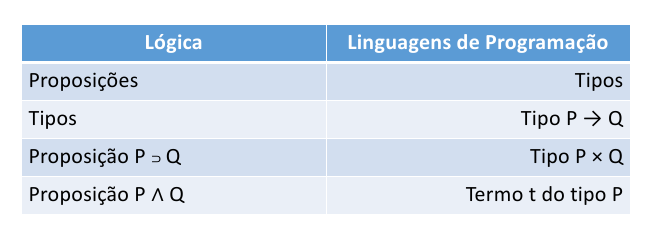
\includegraphics[width=0.65\textwidth]{figuras/tabela.png}
\caption{Tabela}
\label{}
\end{figure}
\end{frame}

\begin{frame}
\frametitle{A correspond�ncia Curry-Howard}
\begin{itemize}
\item A correspond�ncia Curry-Howard n�o �  limitada para um sistema de um tipo particular e uma logica espec�fica, pelo contrario pode ser estendido a uma enorme variedade de sistemas de tipos e l�gicas.
\end{itemize}
\end{frame}

\begin{frame}
\frametitle{Corre��o e Tipagem}
\begin{itemize}
\item Anota��es de tipo n�o desempenham qualquer papel na avalia��o.
\item A maioria dos compiladores para linguagens de programa��o em grande escala, evitam mostrar coment�rios em tempo de execu��o: eles s�o usados durante o typechecking (e durante a gera��o de c�digo, em compiladores mais sofisticados).
\item Tipos n�o aparecem no c�lculo lambda simplesmente tipado na sua forma compilada. Os programas s�o convertidos para uma forma sem tipos antes de serem avaliadas.

\end{itemize}
\end{frame}


%fim camila


\bibliography{referencias}
\bibliographystyle{plainnat}

\end{document}
